% ************************************************************************************************
% **************** Template para la elaboración del libro de Proyecto de Grado,*******************
% ******************** siguiendo los lineamientos establecidos por el ****************************
% ************* Decanato de Estudios Profesionales de la Universidad Simón Bolívar ***************
% *** "Normas para Redacción y Presentación del Libro Final del Proyecto de Grado y Pasantías" ***
% ***************** en la pág. web http://www.profesionales.usb.ve/es/node/4 *********************
% ************************************************************************************************

% ************************************************************************************************
% *** Versión: v1.0                                                                            ***
% *** Autor: Luis Pérez Bustos                                                                 ***
% *** Estudiante de Ingeniería Electrónica                                                     ***
% *** Fecha: 08/04/2017                                                                        ***                      
% *** Licencia: MIT License (c) 2017 Luis Perez Bustos                                         ***
% *** GitHub: https://github.com/lperezbustos/ProyectoDeGrado-Template-USB                     ***
% ************************************************************************************************

\documentclass[letterpaper,12pt,oneside,times,numbered,print,custommargin]{Clases/USB}

% El archivo README.md muestra información necesaria, por favor leerlo.

% ************************************** HEADER *****************************************
% ************************ Packages needed and some configurations **********************
% ***************************************************************************************

% ************************************ MARGINS ******************************************
\usepackage[left=30mm,right=20mm,top=20mm,bottom=20mm]{geometry}

% ************************************** SPANISH ****************************************
\usepackage[spanish,es-lcroman,es-tabla]{babel} % lowercase roman numbers and "Tabla" name
\usepackage[utf8]{inputenc}
\usepackage{fancyhdr}

\fancypagestyle{fan}{ % redefine "fan" style
    \fancyhf{}
    \fancyhead[R]{\thepage} % page number in upper right corner
    \renewcommand{\headrulewidth}{0pt} % without separation line in header
}

\fancypagestyle{fan2}{ % redefine "fan2" style
    \fancyhf{}
    \renewcommand{\headrulewidth}{0pt} % without separation line in header
    \fancyfoot[C]{\thepage}
}

% ********************************* FIGURES ************************************
\usepackage{graphicx}
\usepackage{float} % for image positioning

% ****************************** CITAS TEXTUALES *******************************
\usepackage{csquotes} % quotes
\setquotestyle[mexican]{spanish} % quotation marks --> mexican style

\renewenvironment{displayquote} % over margin for quotes with more than 3 lines
  {\small\list{}{\rightmargin=0.5cm \leftmargin=1.0cm}
   \item\relax}
  {\endlist}
  
\usepackage{epigraph} % epigraph in first page of every chapter
\usepackage{blindtext} % verification text
\usepackage{hyperref} % url

% ********************************** TABLES ************************************
\usepackage[table,xcdraw]{xcolor} % colors for cells and borders
\usepackage{multirow}
\usepackage{tabularx}
\usepackage{adjustbox} % adjust to page size

% ******************************* MATH AND UNITS *******************************
\usepackage{amsfonts}
\usepackage{amsmath}
\usepackage{amssymb}
\usepackage{siunitx} % unidades del sistema internacional

% ****************************** PROGRAMMING CODE ******************************
\usepackage{listings}
\usepackage{color} % color configuration
 
\definecolor{codegreen}{rgb}{0,0.6,0} % some color definitions
\definecolor{codegray}{rgb}{0.5,0.5,0.5} % {RED,GREEN,BLUE}
\definecolor{codepurple}{rgb}{0.58,0,0.82}
\definecolor{backcolour}{rgb}{0.97,0.97,0.97}

\lstdefinestyle{mystyle}{
    backgroundcolor=\color{backcolour},   
    commentstyle=\color{codegreen},
    keywordstyle=\color{blue},
    numberstyle=\tiny\color{codegray},
    stringstyle=\color{black},
    basicstyle=\footnotesize,
    breakatwhitespace=false,         
    breaklines=true,                 
    captionpos=b,                    
    keepspaces=true,                 
    numbers=left,                    
    numbersep=5pt,                  
    showspaces=false,                
    showstringspaces=false,
    showtabs=false,                  
    tabsize=2,
    aboveskip=2em,
    belowskip=2em,
}

\lstset{style=mystyle} % set to style configured behind
\usepackage{chngcntr}

% ************* TITLE FORMAT FOR: CHAPTERS / SECTIONS /SUBSECTIONS  ***********
\RequirePackage{titlesec}
\titleformat{\chapter}[display]{\normalfont\center\bfseries}{\large CAPÍTULO \thechapter}{5pt}{\bfseries}   
\titlespacing*{\chapter}{0pt}{-30pt}{20pt} % delete additional space (-30pt) between title and text

\titleformat{\section}{\normalfont\raggedright\bfseries}{\thesection.}{5pt}{} % section format
\titleformat{\subsection}{\normalfont\raggedright\bfseries}{\thesubsection.}{5pt}{} % subsection format
\titleformat{\subsubsection}{\normalfont\raggedright\bfseries}{\thesubsubsection.}{5pt}{} % sub-subsection format

% ******************* TILE FORMAT FOR: TOC / LOF / LOT  ***********************
\addto\captionsspanish{\renewcommand{\listtablename}{ÍNDICE DE TABLAS}}
\addto\captionsspanish{\renewcommand{\listfigurename}{ÍNDICE DE FIGURAS}}

\usepackage{tocloft} % toc tile format
\renewcommand{\cfttoctitlefont}{\hfill\normalfont\bfseries\MakeUppercase}
\renewcommand{\cftaftertoctitle}{\hfill} % centering title
\renewcommand{\cftaftertoctitleskip}{20pt} % space between title and text
\renewcommand{\cftbeforetoctitleskip}{0cm}
\renewcommand{\cftlottitlefont}{\hfill\normalfont\bfseries}
\renewcommand{\cftafterlottitle}{\hfill} % centering title
\renewcommand{\cftafterlottitleskip}{20pt} % space between title and text
\renewcommand{\cftbeforelottitleskip}{0cm}
\renewcommand{\cftloftitlefont}{\hfill\normalfont\bfseries}
\renewcommand{\cftafterloftitle}{\hfill} % centering title
\renewcommand{\cftafterloftitleskip}{20pt} % space between title and text
\renewcommand{\cftbeforeloftitleskip}{0cm}

%********************************** WATERMARK ***********************************
\usepackage[nostamp]{draftwatermark} % normally off

% to turn off watermark
\makeatletter
\def\watermarkoff{%
        \@sc@wm@stampfalse
}
\makeatother

% to turn on watermark
\makeatletter
\def\watermarkon{%
        \@sc@wm@stamptrue
}
\makeatother

\SetWatermarkAngle{45} % angle to display in page
\SetWatermarkText{Acta de Evaluación} % page 3 in thesis book
\SetWatermarkScale{0.6}
\SetWatermarkLightness{.8}

% *************************** TABLE OF CONTENTS ********************************
\setcounter{secnumdepth}{3} % depth in table of contents
\setcounter{tocdepth}{3}

% ******************************* ABBREVIATIONS ********************************
\usepackage[intoc]{nomencl}
\makenomenclature
\addto\captionsspanish{\renewcommand{\nomname}{LISTA DE ABREVIATURAS}}

% ***************** ABBREVIATIONS AND ACRONYMS LIST ****************************
% ALL THE ABBREVIATIONS AND ACRONYMS HAVE TO BE HERE FOLLOWING THE FORMAT IN SAMPLE
% FOR ACRONYMS IN ANOTHER LANGUAGE, TRANSLATION TO SPANISH MUST APPEARS
\nomenclature{$USB$}{Universidad Simón Bolívar}
\nomenclature{$EC$}{Electronics and Circuits\\Electrónica y Circuitos}
\nomenclature{$...$}{...}
% ******************************* REFERENCES ***********************************
% ** REFERENCE PART NEEDS TO BE IMPROVED TO HAVE EXACTLY USB FORMAT **
\usepackage[backend=biber, maxnames=99, style=numeric-comp, citestyle=numeric, bibstyle=numeric, sorting=none, url=false, natbib=true]{biblatex}
\bibliography{3_BackMatter/Referencias/ref} % Location of references.bib only for biblatex

\DeclareFieldFormat{url}{Disponible en Internet\addcolon\space\url{#1}}
\DeclareFieldFormat[online]{date}{}
% ****************************************************************************** % Preámbulo: configuraciones y paquetes necesarios

% *******************************************************************************
% ******************************** Front Matter *********************************
% *******************************************************************************
\begin{document}

% ***************************************************************************************
% ************************************ CARÁTULA *****************************************
% ***************************************************************************************
\thispagestyle{empty}
\begin{center}

\includegraphics[width=0.20\textwidth]{Figuras/USB_logo.eps}\\ % USB logo
{\large UNIVERSIDAD SIMÓN BOLÍVAR}\\\textbf{DECANATO DE ESTUDIOS PROFESIONALES}\\\textbf{COORDINACIÓN DE ...} % header
\\[8\baselineskip]

%% Titulo del Proyecto de Grado
\textbf{** COLOQUE AQUÍ EL TITULO DE SU PROYECTO DE GRADO **}
\\[2\baselineskip]

%% Author
Por:\\ ** COLOQUE AQUÍ SU NOMBRE **\\ carnet XX-XXXXX
\\[8\baselineskip]

%% some other information
PROYECTO DE GRADO\\Presentado ante la Ilustre Universidad Simón Bolívar\\como requisito parcial para optar al título de \\** TITULO A OBTENER **
\\[2\baselineskip]

%% date and place
\textbf{Sartenejas, ** FECHA **}
\end{center}
% ***************************************************************************************
% ********************************* PÁGINA DE TÍTULO ************************************
% ***************************************************************************************
\thispagestyle{empty}
\begin{center}

\includegraphics[width=0.20\textwidth]{Figuras/USB_logo.eps}\\ % Logo de la Universidad Simon Bolivar
{\large UNIVERSIDAD SIMÓN BOLÍVAR}\\\textbf{DECANATO DE ESTUDIOS PROFESIONALES}\\\textbf{COORDINACIÓN DE ...} % header
\\[8\baselineskip]

%% Titulo del Proyecto de Grado
\textbf{** COLOQUE AQUÍ EL TITULO DE SU PROYECTO DE GRADO **}
\\[2\baselineskip]

%% Author
Por:\\ ** COLOQUE AQUÍ SU NOMBRE **\\ carnet XX-XXXXX
\\[2\baselineskip]

%% Tutor del Proyecto de Grado
Realizado con la asesoría de:\\ Prof. ** TUTOR **
\\[4\baselineskip]

%% some other information
PROYECTO DE GRADO\\Presentado ante la Ilustre Universidad Simón Bolívar\\como requisito parcial para optar al título de \\** TITULO A OBTENER **
\\[2\baselineskip]

%% date and place
\textbf{Sartenejas, ** FECHA **}
\end{center}

% ***************************************************************************************
% ******************************** ACTA DE EVALUACIÓN ***********************************
% ***************************************************************************************
\watermarkon
\chapter*{} % just an unuseful page
\thispagestyle{empty}

\frontmatter
\pagestyle{fan2}    % pagestyle in frontmatter
% ***************************************************************************************
% ************************************* RESUMEN *****************************************
% ***************************************************************************************
% Típicamente el resumen es de las últimas secciones que se escriben
\watermarkoff
\begin{resumen}
\begin{center}
\begin{large}
	UNIVERSIDAD SIMÓN BOLÍVAR
\end{large}

\textbf{DECANATO DE ESTUDIOS PROFESIONALES}

\textbf{COORDINACIÓN DE ...}

~\\
~\\
\textbf{** COLOQUE AQUÍ EL TITULO DE SU PROYECTO DE GRADO **}
~\\
~\\
\textbf{PROYECTO DE GRADO}


Por: ** COLOQUE AQUÍ SU NOMBRE **\\
Realizado con la asesoría de: Prof. ** TUTOR **

~\\

\textbf{RESUMEN}
\end{center}


\setstretch{1.0}

** COLOQUE AQUÍ EL RESUMEN DE SU PROYECTO DE GRADO, APROXIMADAMENTE 250 PALABRAS EN UN SÓLO PÁRRAFO **.

~\\
\textit{\textbf{Palabras clave:}} ** COLOQUE AQUÍ KEYWORDS **.

\setstretch{1.5}
\end{resumen}         % a very organized abstract is important
% ***************************************************************************************
% ************************************ DEDICATORIA **************************************
% ***************************************************************************************

\begin{dedicatoria} 
\\[14\baselineskip]
Gracias por mantenerme a flote en los momentos más difíciles,\\Elizabeth, Edgar Julián, Edgar Augusto y Genesis,\\esto es para ustedes...

\end{dedicatoria}     % just a couple of phrases
% ***************************************************************************************
% ********************************* AGRADECIMIENTOS *************************************
% ***************************************************************************************
\begin{agradecimientos}      

** SOME VERY IMPORTANT ACKNOWLEDGES TO THE PEOPLE THAT HELPED YOU TO ACHIEVE YOUR GOAL AT SIMON BOLIVAR UNIVERSITY. CONGRATULATIONS ! YOU DID IT ! **

\end{agradecimientos}
 % remember the people that helped you


\tableofcontents    % índice general
\newpage
\listoftables       % índice de tablas
\newpage
\listoffigures      % índice de figuras
\newpage

\printnomenclature[2.5cm] % lista de abreviaturas y nomenclatura (ver preambulo.tex)

% *******************************************************************************
% ******************************** Main Matter **********************************
% *******************************************************************************

% ********************************** Introducción *******************************
\mainmatter
\pagestyle{fan} % pagestyle in mainmatter
% ***************************************************************************************
% ************************************ INTRODUCCIÓN *************************************
% ***************************************************************************************
\chapter*{INTRODUCCIÓN}
\addcontentsline{toc}{chapter}{INTRODUCCIÓN}
\thispagestyle{empty}

** COLOQUE CONTENIDO RESPECTIVO AQUÍ **\\

\textbf{Objetivo General:}

\begin{itemize}
    \item ** OBJETIVO GENERAL **.
\end{itemize}

\textbf{Objetivos Específicos:}

\begin{itemize}
    \item ** OBJETIVO ESPECÍFICO 1 **.
    \item ** OBJETIVO ESPECÍFICO 2 **.
    \item ** OBJETIVO ESPECÍFICO 3 **.
    \item ...
\end{itemize}


% ****************************** Cuerpo del Trabajo *****************************
% ***************************************************************************************
% ************************************* CAPÍTULO I **************************************
% ***************************************************************************************
\chapter{** TITULO DEL CAPÍTULO 1 **}
\thispagestyle{empty}

\abovedisplayskip=0pt
\belowdisplayskip=10pt
\abovedisplayshortskip=0pt
\belowdisplayshortskip=10pt

\epigraph{\flushright El auténtico pensar, como el vivir, es tarea que se aprende. Quien aprende, debe dialogar con
aquellos que han pensado previamente: recorrer sus itinerarios, seguir sus rutas y estelas, consultar
sus bitácoras}{\textit{Ernesto Mayz Vallenilla}\\Rector fundador de la USB}

** COLOQUE AQUÍ CONTENIDO RESPECTIVO **\\

** A CONTINUACIÓN SE HACE UN RESUMEN DE LAS PRINCIPALES HERRAMIENTAS NECESARIAS PARA ESCRIBIR SU LIBRO DE PROYECTO DE GRADO. EL OBJETIVO DE ESTO ES AHORRAR LA MAYOR CANTIDAD DE TIEMPO EN EL \textit{LAYOUT}, ENFOCANDO LOS ESFUERZOS EN EL CONTENIDO DEL PROYECTO **

\section{Figures}

\subsection{Referenciado y posicionamiento de imagenes}

En la figura \ref{fig:cromovegetal} se observa el jardín cromovegetal, concebido por Carlos Cruz-Diez en 1991 en su visita a la Universidad Simón Bolívar.

% for a correct image positioning is important to use the parameters [H], [h] and [p] in a right way.
% The first one place the image in the exact position that is in the LaTeX code
% The second one place the image where the compiler configurate as "best position"
% The last one utilize an entire page for figure positioning

\begin{figure}[H]
\centering
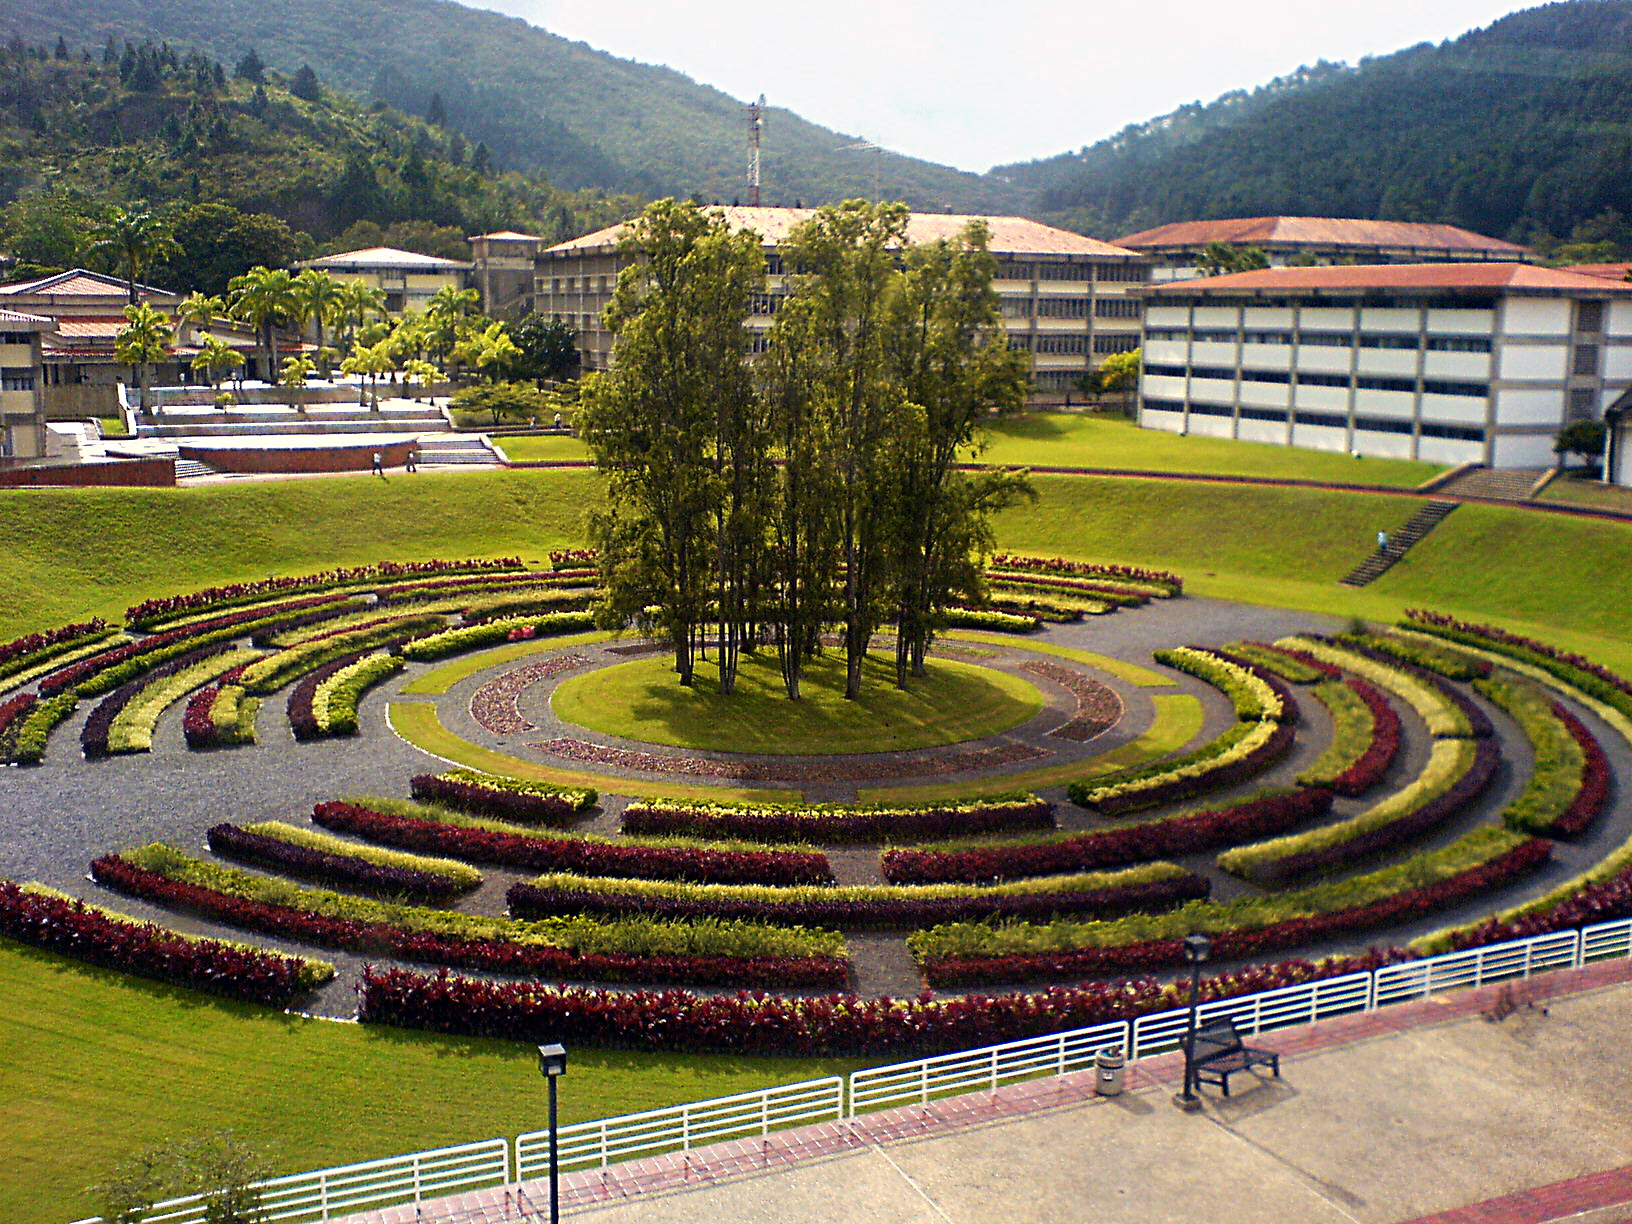
\includegraphics[width=0.50\textwidth]{2_MainMatter/Capitulo1/Imagenes/cromovegetal.jpg}
\caption{Jardín cromovegetal de la Universidad Simón Bolívar}
\label{fig:cromovegetal}
\end{figure}

\subsection{Ejemplo de posicionamiento en hoja completa}

La figura \ref{fig:rectorado} muestra el rectorado de la Universidad Simón Bolívar, sede de los principales entes administrativos de la institución.

\begin{figure}[p]
\centering
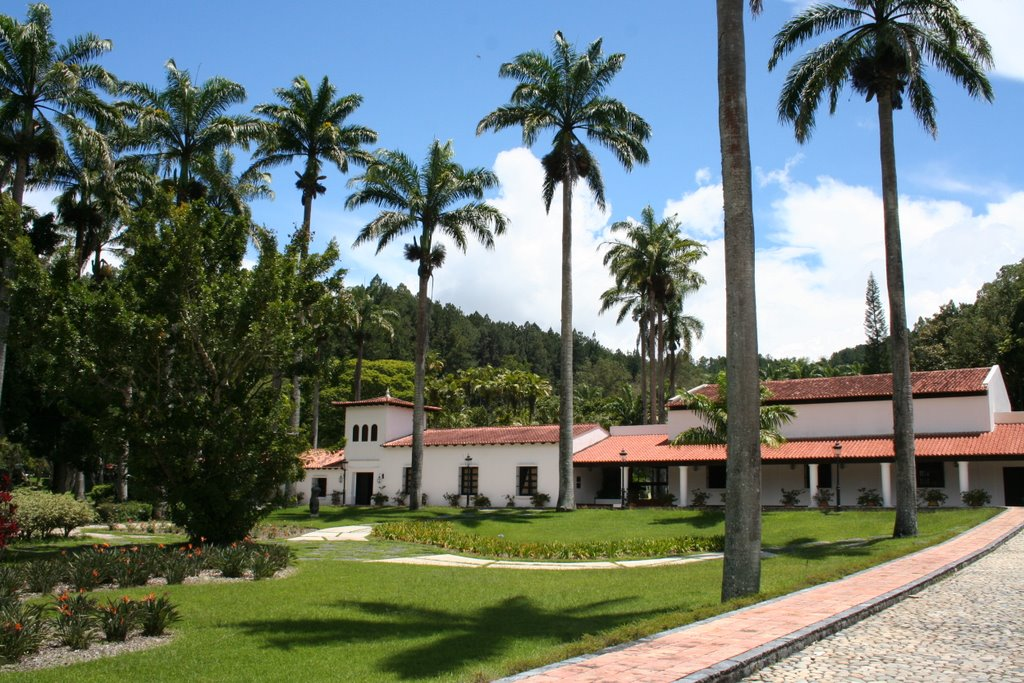
\includegraphics[width=1.0\textwidth]{2_MainMatter/Capitulo1/Imagenes/rectorado.jpg}
\caption{Rectorado de la Universidad Simón Bolívar}
\label{fig:rectorado}
\end{figure}

\subsection{Ángulo de giro en imágenes con orientación horizontal}

La figura \ref{fig:biblioteca} muestra la biblioteca de la USB, lugar de estudio e investigación de un gran número de miembros de la comunidad universitaria.

\begin{figure}[p]
\centering
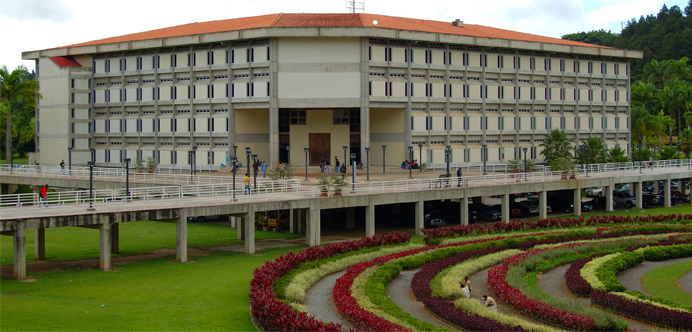
\includegraphics[width=1.3\textwidth, angle=90]{2_MainMatter/Capitulo1/Imagenes/biblioteca.jpg}
\caption{Biblioteca de la Universidad Simón Bolívar}
\label{fig:biblioteca}
\end{figure}

\section{Quotes}

\section{Tables}

\section{Equations}

\section{Programming Code}

\section{Referencias}
% ***************************************************************************************
% ************************************* CAPÍTULO II *************************************
% ***************************************************************************************
\chapter{** TITULO DEL CAPÍTULO 2 **}
\thispagestyle{empty}

\epigraph{\flushright Simplicidad es un prerequisito de confiabilidad}{\textit{Edsger W. Dijkstra}}

** COLOQUE AQUÍ EL CONTENIDO RESPECTIVO DEL CAPÍTULO 2 **
% ***************************************************************************************
% ************************************ CAPÍTULO III *************************************
% ***************************************************************************************
\chapter{** TITULO DEL CAPÍTULO 3 **}
\thispagestyle{empty}

\epigraph{\flushright Nunca alguna gran obra se ha hecho de prisa. Lograr un gran descubrimiento científico, imprimir una excelente fotografía, escribir un poema inmortal... hacer cualquier gran logro requiere tiempo, paciencia y perseverancia}{\textit{W. J. Wilmont Buxton}}

** COLOQUE AQUÍ EL CONTENIDO RESPECTIVO DEL CAPÍTULO 3 **
% ***************************************************************************************
% ************************************* CAPÍTULO IV *************************************
% ***************************************************************************************
\chapter{** TITULO DEL CAPÍTULO 4 **}
\thispagestyle{empty}

\epigraph{\flushright Si buscas resultados distintos no hagas siempre lo mismo}{\textit{Albert Einstein}}

** COLOQUE AQUÍ EL CONTENIDO RESPECTIVO DEL CAPÍTULO 4 **
% .
% .
% .
% \include{2_MainMatter/CapituloN/capN}

% ********************************** Conclusiones *******************************
% ***************************************************************************************
% ********************************** CONCLUSIONES ***************************************
% ***************************************************************************************
\chapter*{CONCLUSIONES Y RECOMENDACIONES}
\thispagestyle{empty}
\addcontentsline{toc}{chapter}{CONCLUSIONES Y RECOMENDACIONES}

\renewcommand{\thefigure}{C.\arabic{figure}}
\setcounter{figure}{0}

\epigraph{\flushright La web, tal como yo la imaginaba, todavía no la hemos visto. El futuro sigue siendo mucho más grande que el pasado}{\textit{Tim Berners-Lee}}

** COLOQUE AQUÍ SU CONTENIDO **

% *******************************************************************************
% ********************************** Back Matter ********************************
% *******************************************************************************

% ********************************** Referencias ********************************

\begin{spacing}{1}          % espaciado reglamentario
\printbibliography[heading=bibintoc, title=REFERENCIAS]
\end{spacing}

% ********************************** Apéndices ********************************
\appendix
% ***************************************************************************************
% ************************************** APÉNDICE A *************************************
% ***************************************************************************************
\chapter*{APÉNDICE A:\\ ** TITULO DEL APÉNDICE **}
\thispagestyle{empty}
\addcontentsline{toc}{chapter}{APÉNDICE A}

\renewcommand{\thefigure}{A.\arabic{figure}}
\setcounter{figure}{0}

\titlespacing\section{0pt}{12pt plus 4pt minus 2pt}{0pt plus 2pt minus 2pt}
\titlespacing\subsection{0pt}{12pt plus 4pt minus 2pt}{0pt plus 2pt minus 2pt}

** AQUÍ EMPIEZA EL APÉNDICE A **
% ***************************************************************************************
% ************************************** APÉNDICE B *************************************
% ***************************************************************************************
\chapter*{APÉNDICE B:\\ ** TITULO DEL APÉNDICE **}
\thispagestyle{empty}
\addcontentsline{toc}{chapter}{APÉNDICE B}

** AQUÍ EMPIEZA EL APÉNDICE B **
% ***************************************************************************************
% ************************************** APÉNDICE C *************************************
% ***************************************************************************************
\chapter*{APÉNDICE C:\\ ** TITULO DEL APÉNDICE **}
\thispagestyle{empty}
\addcontentsline{toc}{chapter}{APÉNDICE C}

** AQUÍ EMPIEZA EL APÉNDICE C **
% .
% .
% .
% \include{3_BackMatter/Apendices/apendiceN}

% *******************************************************************************
% *************************************** END ***********************************
% *******************************************************************************

\end{document}
